\section{Auswertung}
\subsection{Messung der PSF}
Zur Bestimmung der Form der PSF werden Aufnahmen, der xy-, xz, und yz-Ebene der Golbeads verwendet. 
Dabei wird jeweils die Ausdehnung des Bildes in x-,y- und z-Richtung bestimmt.
Da die Goldkügelchen in erster Näherung als rund angenommen werden können, ist die Form der PSF theoretisch bekannt.
Sie folgt der Besselfunktion $J_1$, für die Beugung von Licht an einer Kreisblende.
Dieses Interferenzmuster kann angenähert werden durch die Funktion \ref{eq:psfapprox}
\begin{align}
	f(x)=I_0 \cdot \exp \left( -k \cdot x^2 \right) \cdot \cos \left(-\omega\cdot x\right). \label{eq:psfapprox}
\end{align}
\\ 
Die Ausdehnung der Airyscheibe entspricht nach dem Rayleigh-Kriterium dem Abstand der beiden ersten Minima voneinander. 
Durch (\ref{eq:psfapprox}) ist der Abstand des ersten Minimums vom ersten Maximum eindeutig mit dem Parameter $w$ bestimmt als:
\begin{align}
x_{min} = \frac{\pi}{2}\omega.
\end{align}
Die PSF wird mit ImageJ vermessen indem das Profil entlang der jeweiligen Achse durch das Maximum bestimmt wird.
In Abb. \ref{fig:psffits} sind die alle Vermessungen der PSF zu sehen. In Tab. \ref{tab:psffits} sind die durch nonlinear-regression bestimmten Werte aufgetragen, der Fehler ergibt sich aus der bei der Regression auftretenden Standartabweichung.
\\
Die aus dem Aufbau nach (\ref{eq:rayleigh}) bestimmte Airyscheibe hat einen Durchmesser von 557.7~nm für eine Wellenlänge von 640~nm und 675.4~nm für eine Wellenlänge von 775~nm.
\\
Bei der Messung der Auslöschung der FLuoreszenz durch den STED-Laser wird eine konfokale Lochblende mit einem Durchmesser von 62.5~$\mu$m und einer 100-fachen Vergrößerung des Bildes benutzt. 
Dies entspricht dem 1.12-fachen Durchmesser der Airyscheibe für 640~nm und 0.92-fachen Durchmesser der Airyscheibe für 775~nm.
\\ 
Ein geringerer Fehler der Messung der Ausdehnung der PSF ist für den Fit mit einer reinen Gaußfunktion zu erwarten, da die Minima nur sehr schwach ausgeprägt sind. 
In diesem Fall lässt sich die FWHM durch die Gaußfunktion bestimmen.
Die bestimmten Werte für die FWHM sind in Tab. \ref{tab:psffwhm} abzulesen. Eine Übersicht der gemessenen Profile mit zugehörigen Fits ist in Abb. \ref{fig:gaussfits} zu finden.
Die sich aus dem Aufbau ergebenden Werte sind in Tab. \ref{tab:fwhmaufbau} zu sehen.
\begin{figure}
	\centering
	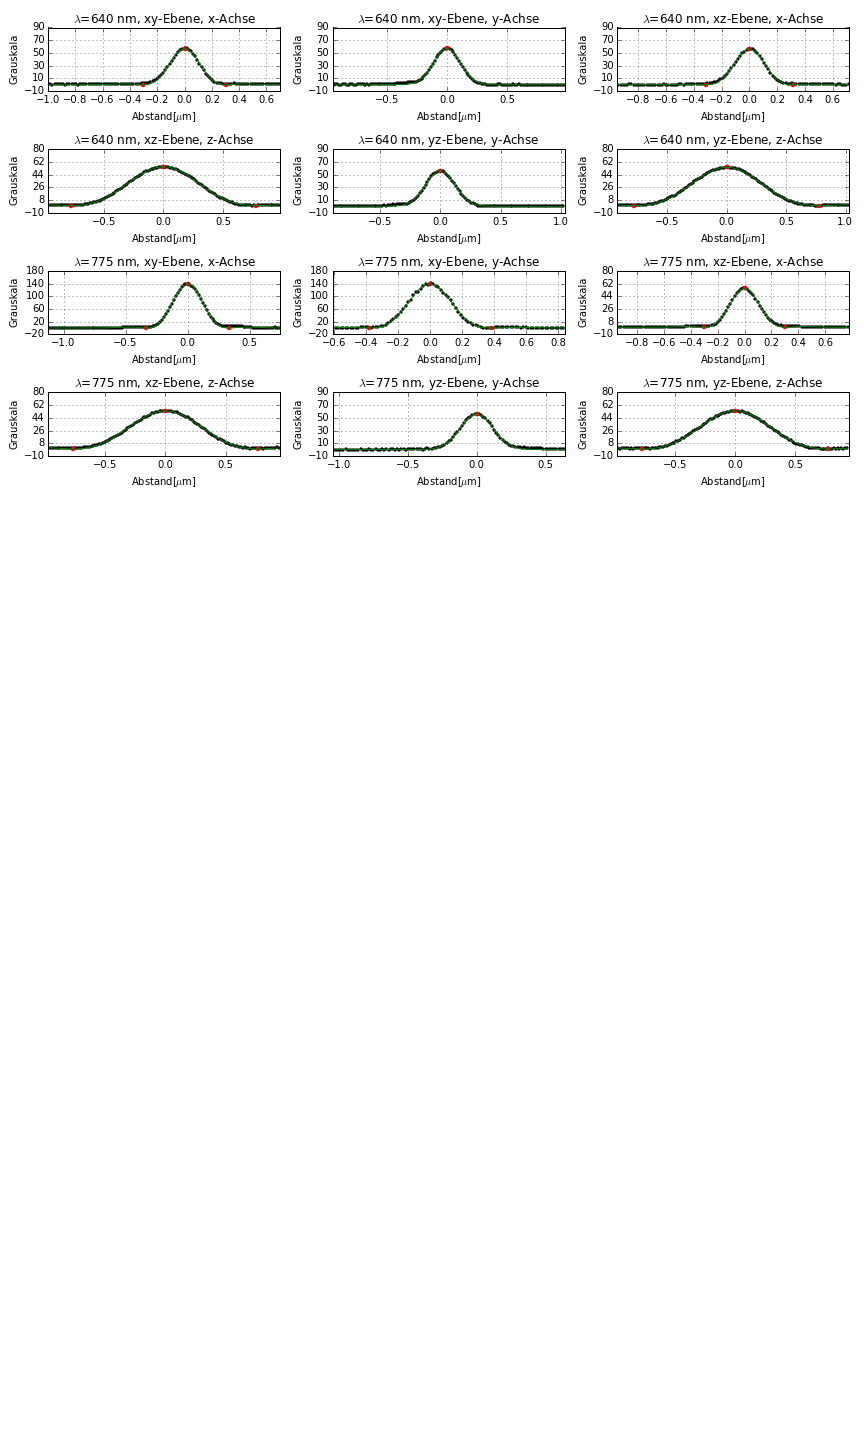
\includegraphics[trim= 0 950 0 0, width=\textwidth]{plots/goldbeads.png}
	\caption{Verteilung der Intensität der Aufnahmen, als Funktion des Abstandes vom ersten Maximum. Mit ImageJ bestimmte Werte sind schwarz dargestellt. 
		Maxima und erste Minima sind in rot hervorgehoben. 
		Die gefittete Funktion (grün) entspricht Gleichung (\ref{eq:psfapprox}). 
		Für die Messungen der y-Achse für die Wellenlängen 640~nm und 775~nm, liefert diese Methode der bestimmung der Minima keine sinnvollen Ergebnisse.
	}\label{fig:psffits}
\end{figure}
\begin{table}
	\centering
	\caption{
		Gewichtete Mittelwerte der Messungen des Durchmessers der Airyscheibe.
Für die $y$-Achse bei $\lambda = 640$~nm ist der Fehler der Regression viel größer als der bestimmte Durchmesser, der weit außerhalb der betrachteten Region liegen würde.
Bei der $\lambda = 775$~nm Messung hat nur ein Fit ein sinnvolles Ergebnis erzielt.}
	% Python latex table
	\begin{tabular}{l|l|c}
		Wellenlänge~[nm] & Achse & Durchmesser der Airyscheibe~[$\mu$m] \\ \hline 
		    &x&0.610(5)\\
		 640&y&--\\ 
		    &z&1.557(4)\\ \hline
		    &x&0.639(5)\\
		 775&y&0.761(8)\\
		    &z&1.546(8)\\
	\end{tabular}\label{tab:psffits}
\end{table}
\begin{table}
\centering
\caption{Durch einen Fit mit einer Gaußfunktion bestimmte Werte für die FWHM des Anregungs- und STED-Lasers. Gezeigt ist der gewichtete Mittelwert, mit einem Fehler der sich aus der Regression ergibt.}\label{tab:psffwhm}
\begin{tabular}{l|l|c}
	Wellenlänge [nm]& Achse & FWHM [nm] \\ \hline
	   &x&244.3(6)\\
	640&y&276.5(5)\\
	   &z&637.2(2)\\ \hline
	   &x&258.0(5)\\
	775&y&291.3(5)\\
	   &z&637.1(2)\\
\end{tabular}
\end{table}
\begin{table}
	\centering
	\caption{Werte für die FWHM der PSF, wie sie durch die Parameter des Aufbaus vorgegeben sind ($NA=1.4$). Die optische Schichtdicke $d_{schicht}$ wurde nach Gl. (\ref{eq:slice}) bestimmt mit einem Pinholedurchmesser von $PH = 625$~nm.}\label{tab:fwhmaufbau}
	\begin{tabular}{l|rr}
		Wellenlänge~[nm] & FWHM~[nm] & $d_{schicht}$ [nm]\\ \hline
		640(lateral/axial) & 233.14/606.86 & 1135.4\\
		775(lateral/axial) & 282.32/734.87 & 1208.7
	\end{tabular}
\end{table}

\subsection{Tiefendiskriminierung}
In Abb. \ref{fig:tiefe} ist der Intensitätsverlauf in Abhängigkeit von der $z$-Achse entlang der Farbfilmprobe dargestellt.
Die Tiefendiskriminierung kann durch die Breite des Intensitätsabfalls abgeschätzt werden.
Weil das Plateau der maximalen Intensität nicht exakt konstant ist wurde für den maximalen Wert der Mittellwert des Plateaus gebildet.
Dafür wurde in Abb. \ref{fig:tiefe} nur der Bereich zwischen den eingezeichneten roten Linien benutzt.
Die Tiefendiskriminierung entspricht in etwa der Länge nach dem die Intensität auf die Hälfte ihres ursprünglichen Wertes abgefallen ist.
In der Abbildung ist dies der Abstand des rechten Randes des Plateaus zur vertikalen gelben Linie.
Der so bestimmte Wert ergibt sich zu 532.5~nm.

\begin{figure}
	\centering
	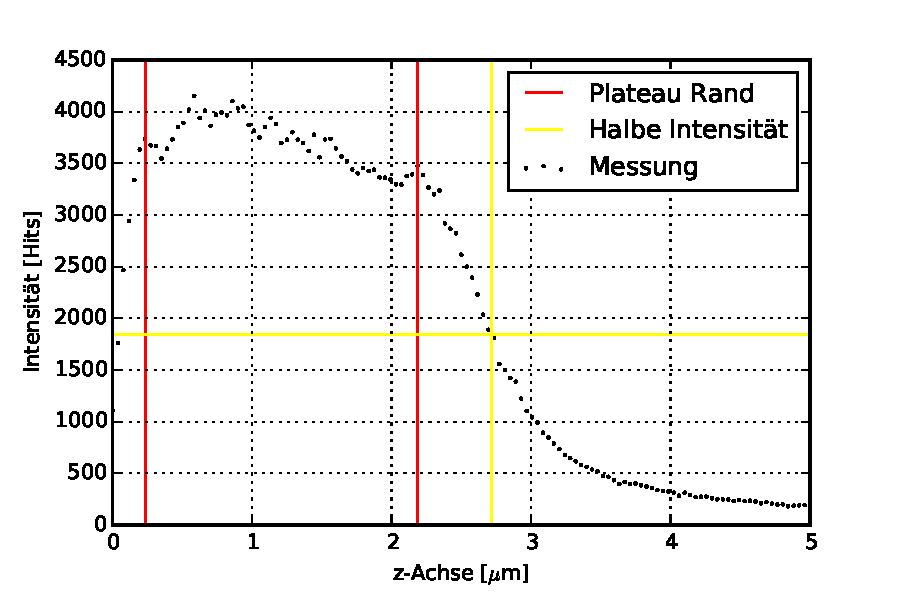
\includegraphics[width=0.6\textwidth]{plots/tiefe.pdf}
	\caption{Verlauf der gemessenen Intensität beim Scannen des Farbfilms entlang der $z$-Achse. Die Intensität entspricht der Anzahl der detektierten Photonen im Photomultiplier.
		Die roten Linien markieren die Grenzen des Plateaus. 
		Die horizontale gelbe Linie beschreibt die Höhe der halben Plateauintensität, und die vertikale gelbe Linie markiert die $z$-Koordinate bei dem dieser Wert erreicht ist.
		Aus dem Abstand des Plateaus von der halben Intensität lässt sich die Tiefendiskriminierung abschätzen.
	}\label{fig:tiefe}
\end{figure}
\newpage
\subsection{STED-Auslöschung}
Zu quantitativen Beschreibung der Auslöschung der Fluoreszenz durch den STED-Laser wird das Verhältnis der gemessenen Intensität ohne Auslöschung zur Intensität mit Auslöschung berechnet.
Aus den Messwerten für die Intensitäten werden die Mittelwerte gebildet, wodurch auch der Effekt der Bleichung der Nanopartikel auf die Messung gemindert wird.
\\
Für die Sättigungsintensität ergibt sich ein Wert von $I_S = 3.2$~MW/cm$^2$.
\begin{figure}
	\centering
	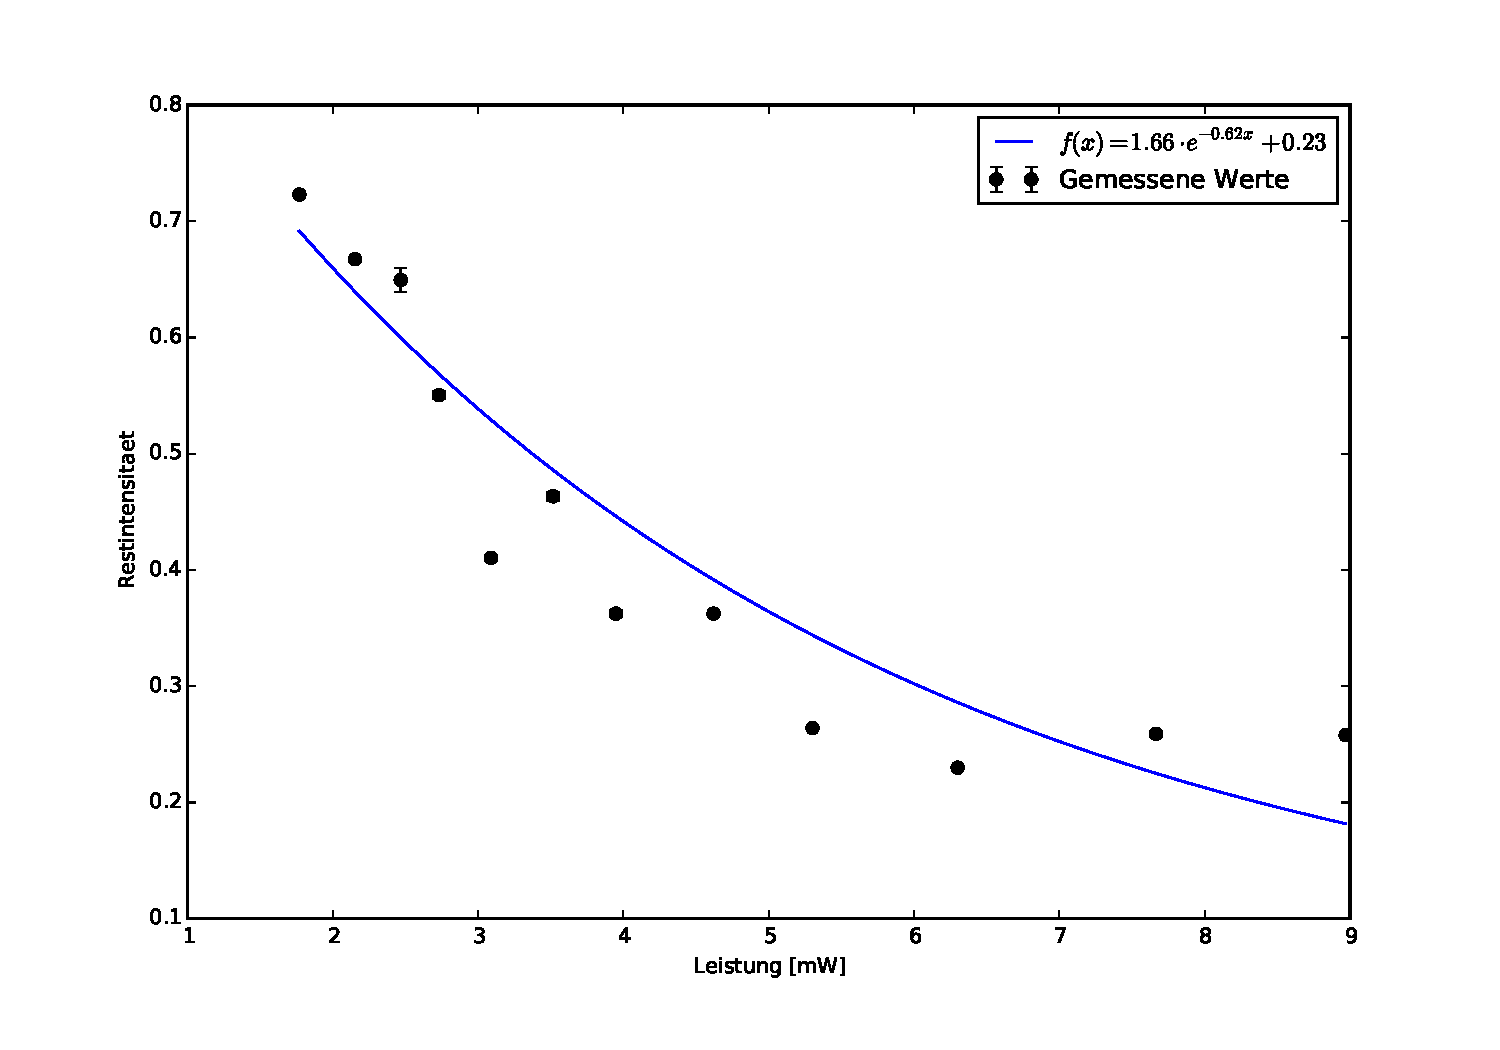
\includegraphics[width=0.75\textwidth]{plots/depletion.pdf}
	\caption{Restintensität als Anteil der Anregungsintensität für verschiedene STED-Leistungen. 
		Die Fehlerbalken ergeben sich aus der Standardabweichung der einzelnen Messungen für eine gegebene STED-Leistung und Beleuchtungsart. 
		Die Messung der Intensität bei Beleuchtung duch den Anregungslaser allein ergibt vier Messwerte je STED-Leistung, und die Messung der Intensität bei gleichzeitiger Beleuchtung mit Anregungs- und STED-Laser liefert zwei Messwerte.
		Die Sättigungsintensität $I_S$ wurde über Interpolation der Messwerte bestimmt. 
		Sie liegt bei $I_S = 3.2$~MW/cm$^2$.
}\label{fig:depletion}
\end{figure}

\subsection{Auflösung der STED-Mikroskopie}
\begin{figure}
	\centering
	\begin{subfigure}{0.3\textwidth	}
		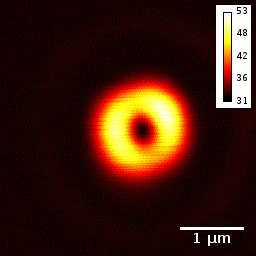
\includegraphics[width=\textwidth]{plots/GoldBeads_3d_775nmxywithbar.jpg}
		\caption{$xy$-Ebene.}
	\end{subfigure}
	~
	\begin{subfigure}{0.3\textwidth	}
		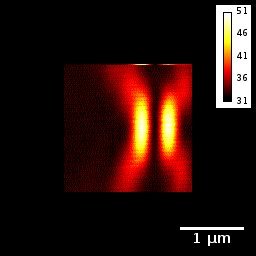
\includegraphics[width=\textwidth]{plots/GoldBeads_3d_775nmxzwithbar.jpg}
		\caption{$xz$-Ebene.}
	\end{subfigure}
	~
	\begin{subfigure}{0.3\textwidth	}
		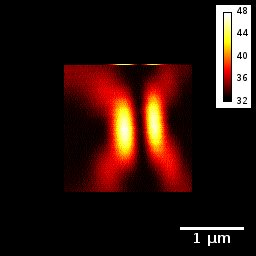
\includegraphics[width=\textwidth]{plots/GoldBeads_3d_775nmyzwithbar.jpg}
		\caption{$yz$-Ebene.}
	\end{subfigure}
	\caption{Aufnahmen der PSF des STED-Lasers, unter Einsatz der Phasenplatte.}\label{fig:doughnut_psf}
\end{figure}
Zunächst wird der STED-Ring untersucht und das Verhältnis der Maximalintensität zur Intensität in der Mitte des Ringes gebildet.
Die Aufnahmen der PSF des STED-Lasers können in Abb. \ref{fig:doughnut_psf} betrachtet werden.
Dazu wird der Intensitätsverlauf entlang der Achse durch Minimum und Maximum des Ringes untersucht. Dieser ist in Abb. \ref{fig:doughnut} zu sehen.
Es ist zu erkennen, dass die Intensität in der Mitte des Ringes vollständig auf den Wert des Hintergrundes abfällt.
In Abb. \ref{fig:doughnut} ist dieser gelb unterlegt.
Die Differenz zwischen Maximum und Minimum beträgt ca. 38~\% der maximalen Intensität. 
\begin{figure}
	\centering
	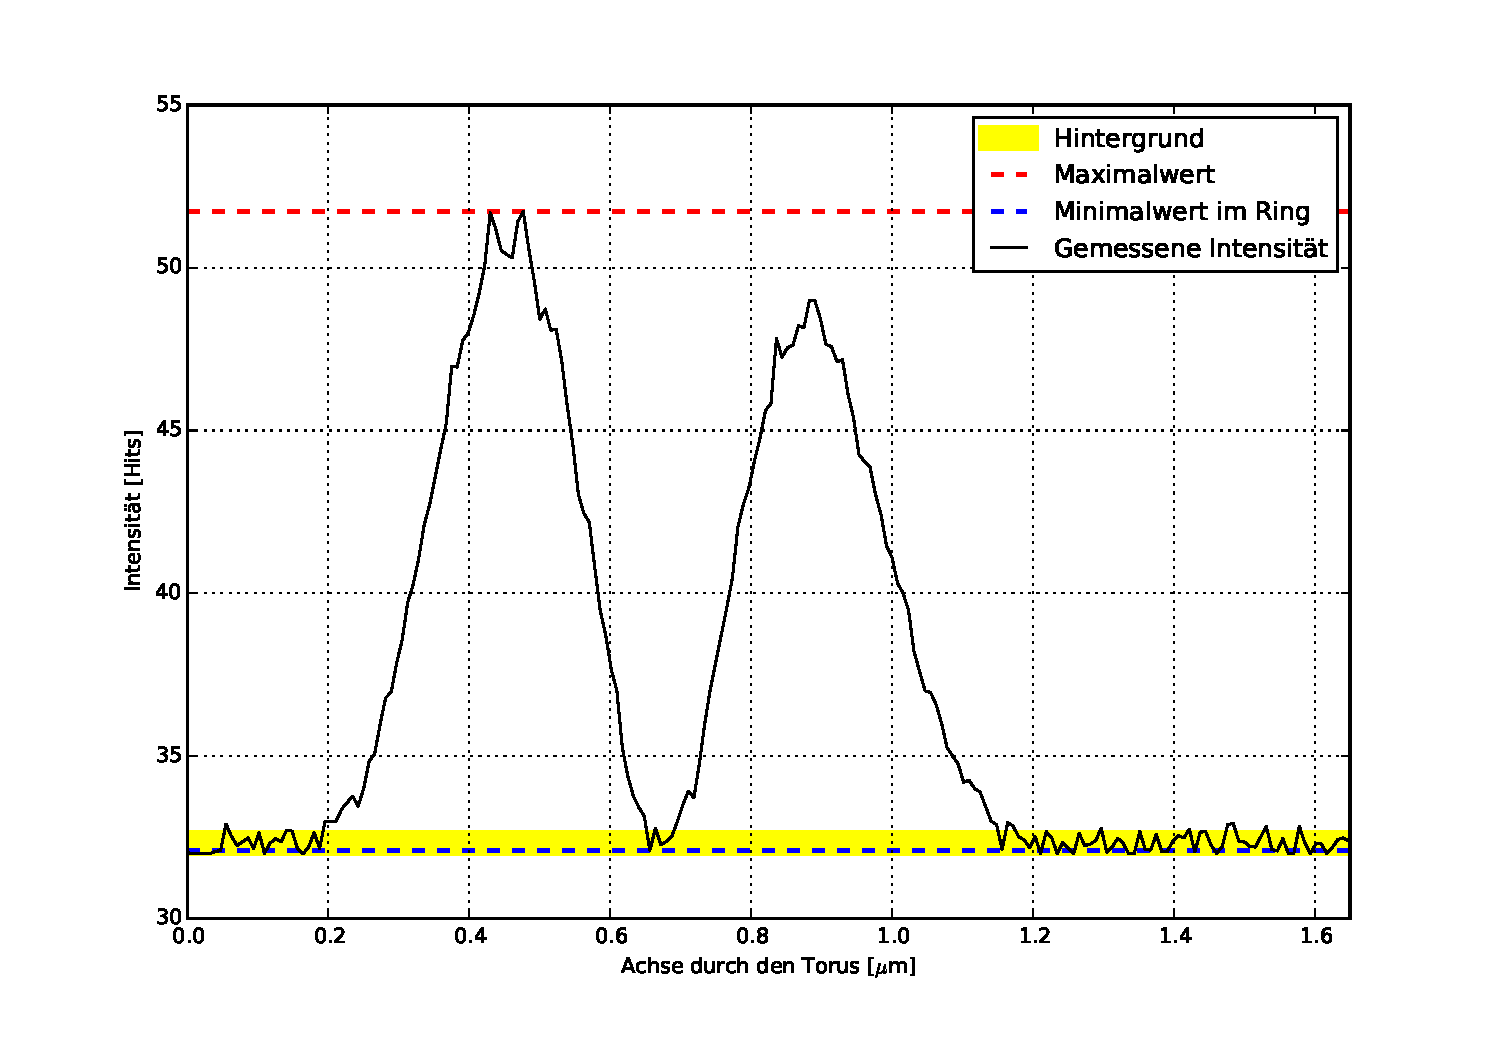
\includegraphics[width=0.75\textwidth]{plots/doughnut.pdf}
	\caption{Intensitätsverlauf entlang der Achse durch den Maximalwert des Ringes und dem Mittelpunkt.
	Die Intensität des Minimums entspricht dem Niveau der Intensität außerhalb des Ringes.}
	\label{fig:doughnut}
\end{figure}
\\ 
Die Auflösung der STED-Mikroskopie wird unter Verwendung des ImageJ Plugins \emph{MosaicSuite} und der darin befindlichen Funktion PSF-Tool bestimmt.\\
Dieses Werkzeug erlaubt die Bestimmung der FWHM einer Aufnahme oder eines gesamten Aufbaus, durch die Berechnung der PSF, die durch einzelne isolierte Punkte erzeugt wird.
Die PSFs mehrerer Nanopartikel wird dann gemittelt und daraus der Mittelwert der FWHMs bestimmt.
\\
Die so bestimmten Werte für die FWHM sind als Funktion der relativen STED-Intensität $\zeta = I_{STED}/I_S$ in Abb. \ref{fig:sted_res} aufgetragen.
Ersetzt man in Gleichung (\ref{eq:sted_res}) den Term $\frac{\lambda}{2NA}$ durch die konofkale Auflösung, und modelliert den Einfluss aller nicht spektroskopischen Parameter auf die Auflösung als einen zur Intensität beitragenden Faktor, so ergibt sich die Funktion (\ref{eq:d-fit}):
\begin{align}
	d = \frac{d_{konfokal}}{\sqrt{1+k^2\zeta}}, \label{eq:d-fit}
\end{align}
Der Fit dieser Funktion an die Messwerte ergibt einen Wert von $k=0.56(8)$.
\begin{figure}
	\centering
	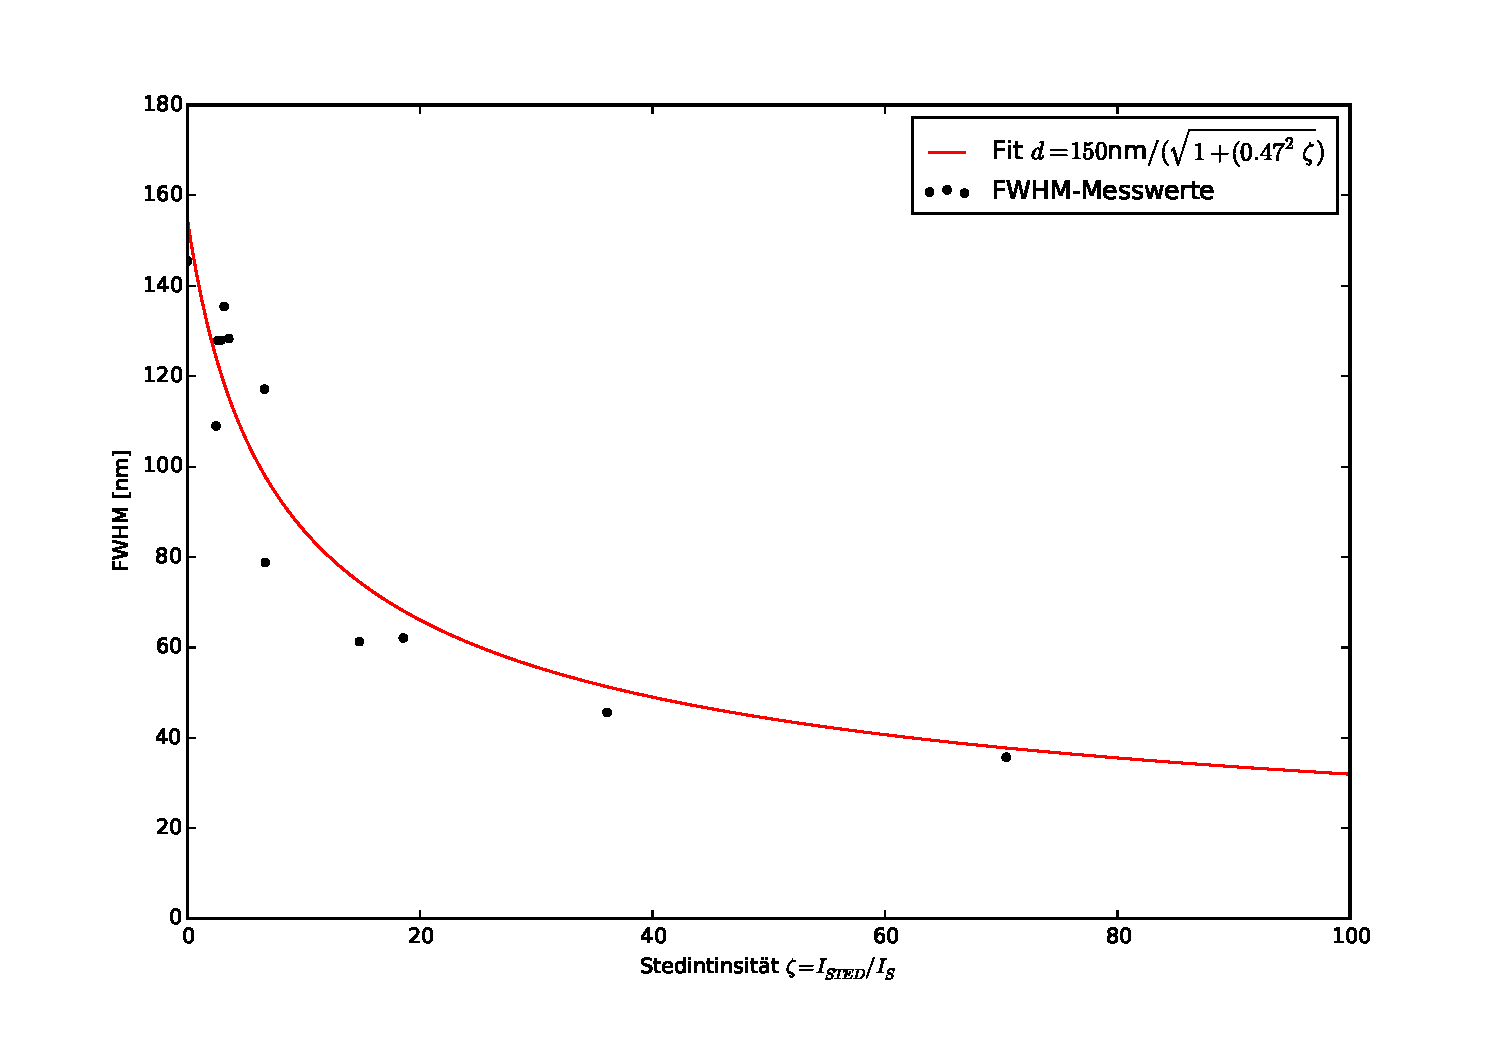
\includegraphics[width=0.75\textwidth]{plots/fwhm_zeta.pdf}
	\caption{FWHM als Funktion der Intensität des STED-Lasers. Der Fit führt zu den Ergebnissen $k = 0.56(8)$ und $d_{konfokal} = 1500(100)$~nm. 
	}\label{fig:sted_res}
\end{figure}

\subsection{Untersuchung der Mikrotubuli}
In Abb. \ref{fig:nosted} bis \ref{fig:tubuli_sted} sind mit dem Aufbau aufgenommene Bilder der Mikrotubuli zu sehen.

\begin{figure}
\centering
\begin{subfigure}{0.3\textwidth}
	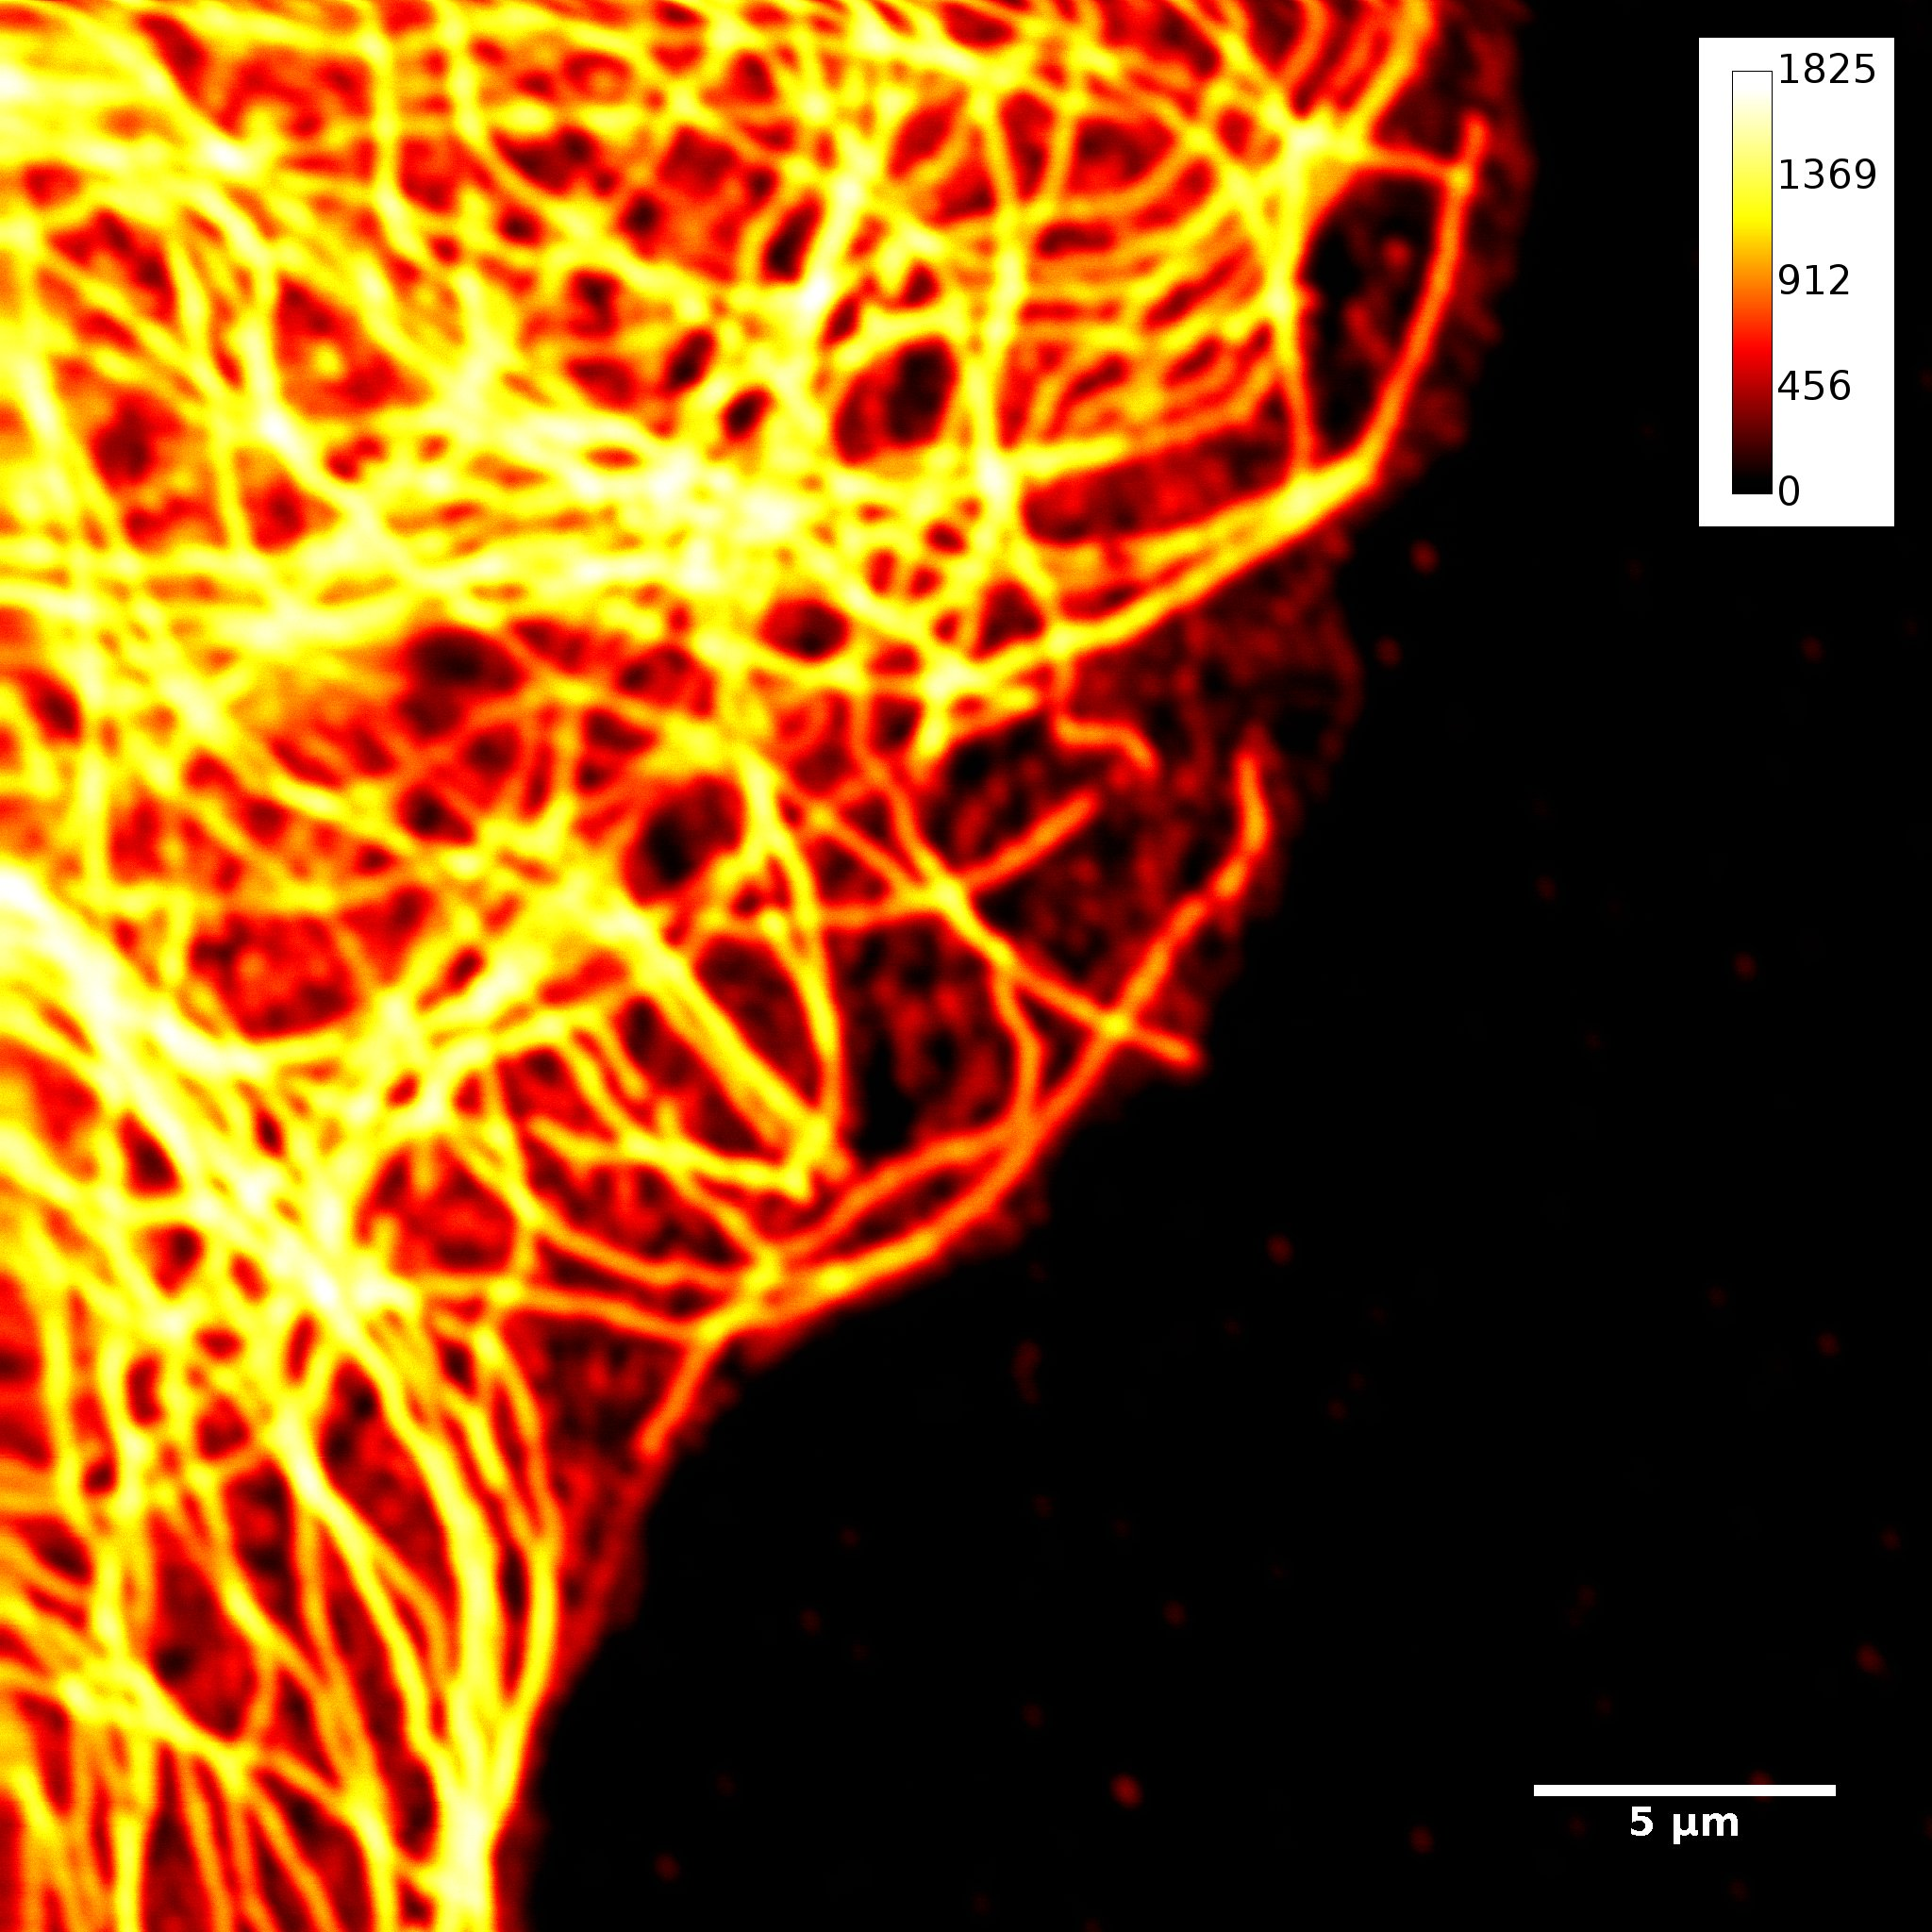
\includegraphics[width=\textwidth]{plots/normal_noSTED_measurement_with_bar.jpg}
	\caption{Anregungslaser allein.}\label{fig:nosted}
\end{subfigure}
~
\begin{subfigure}{0.3\textwidth}
	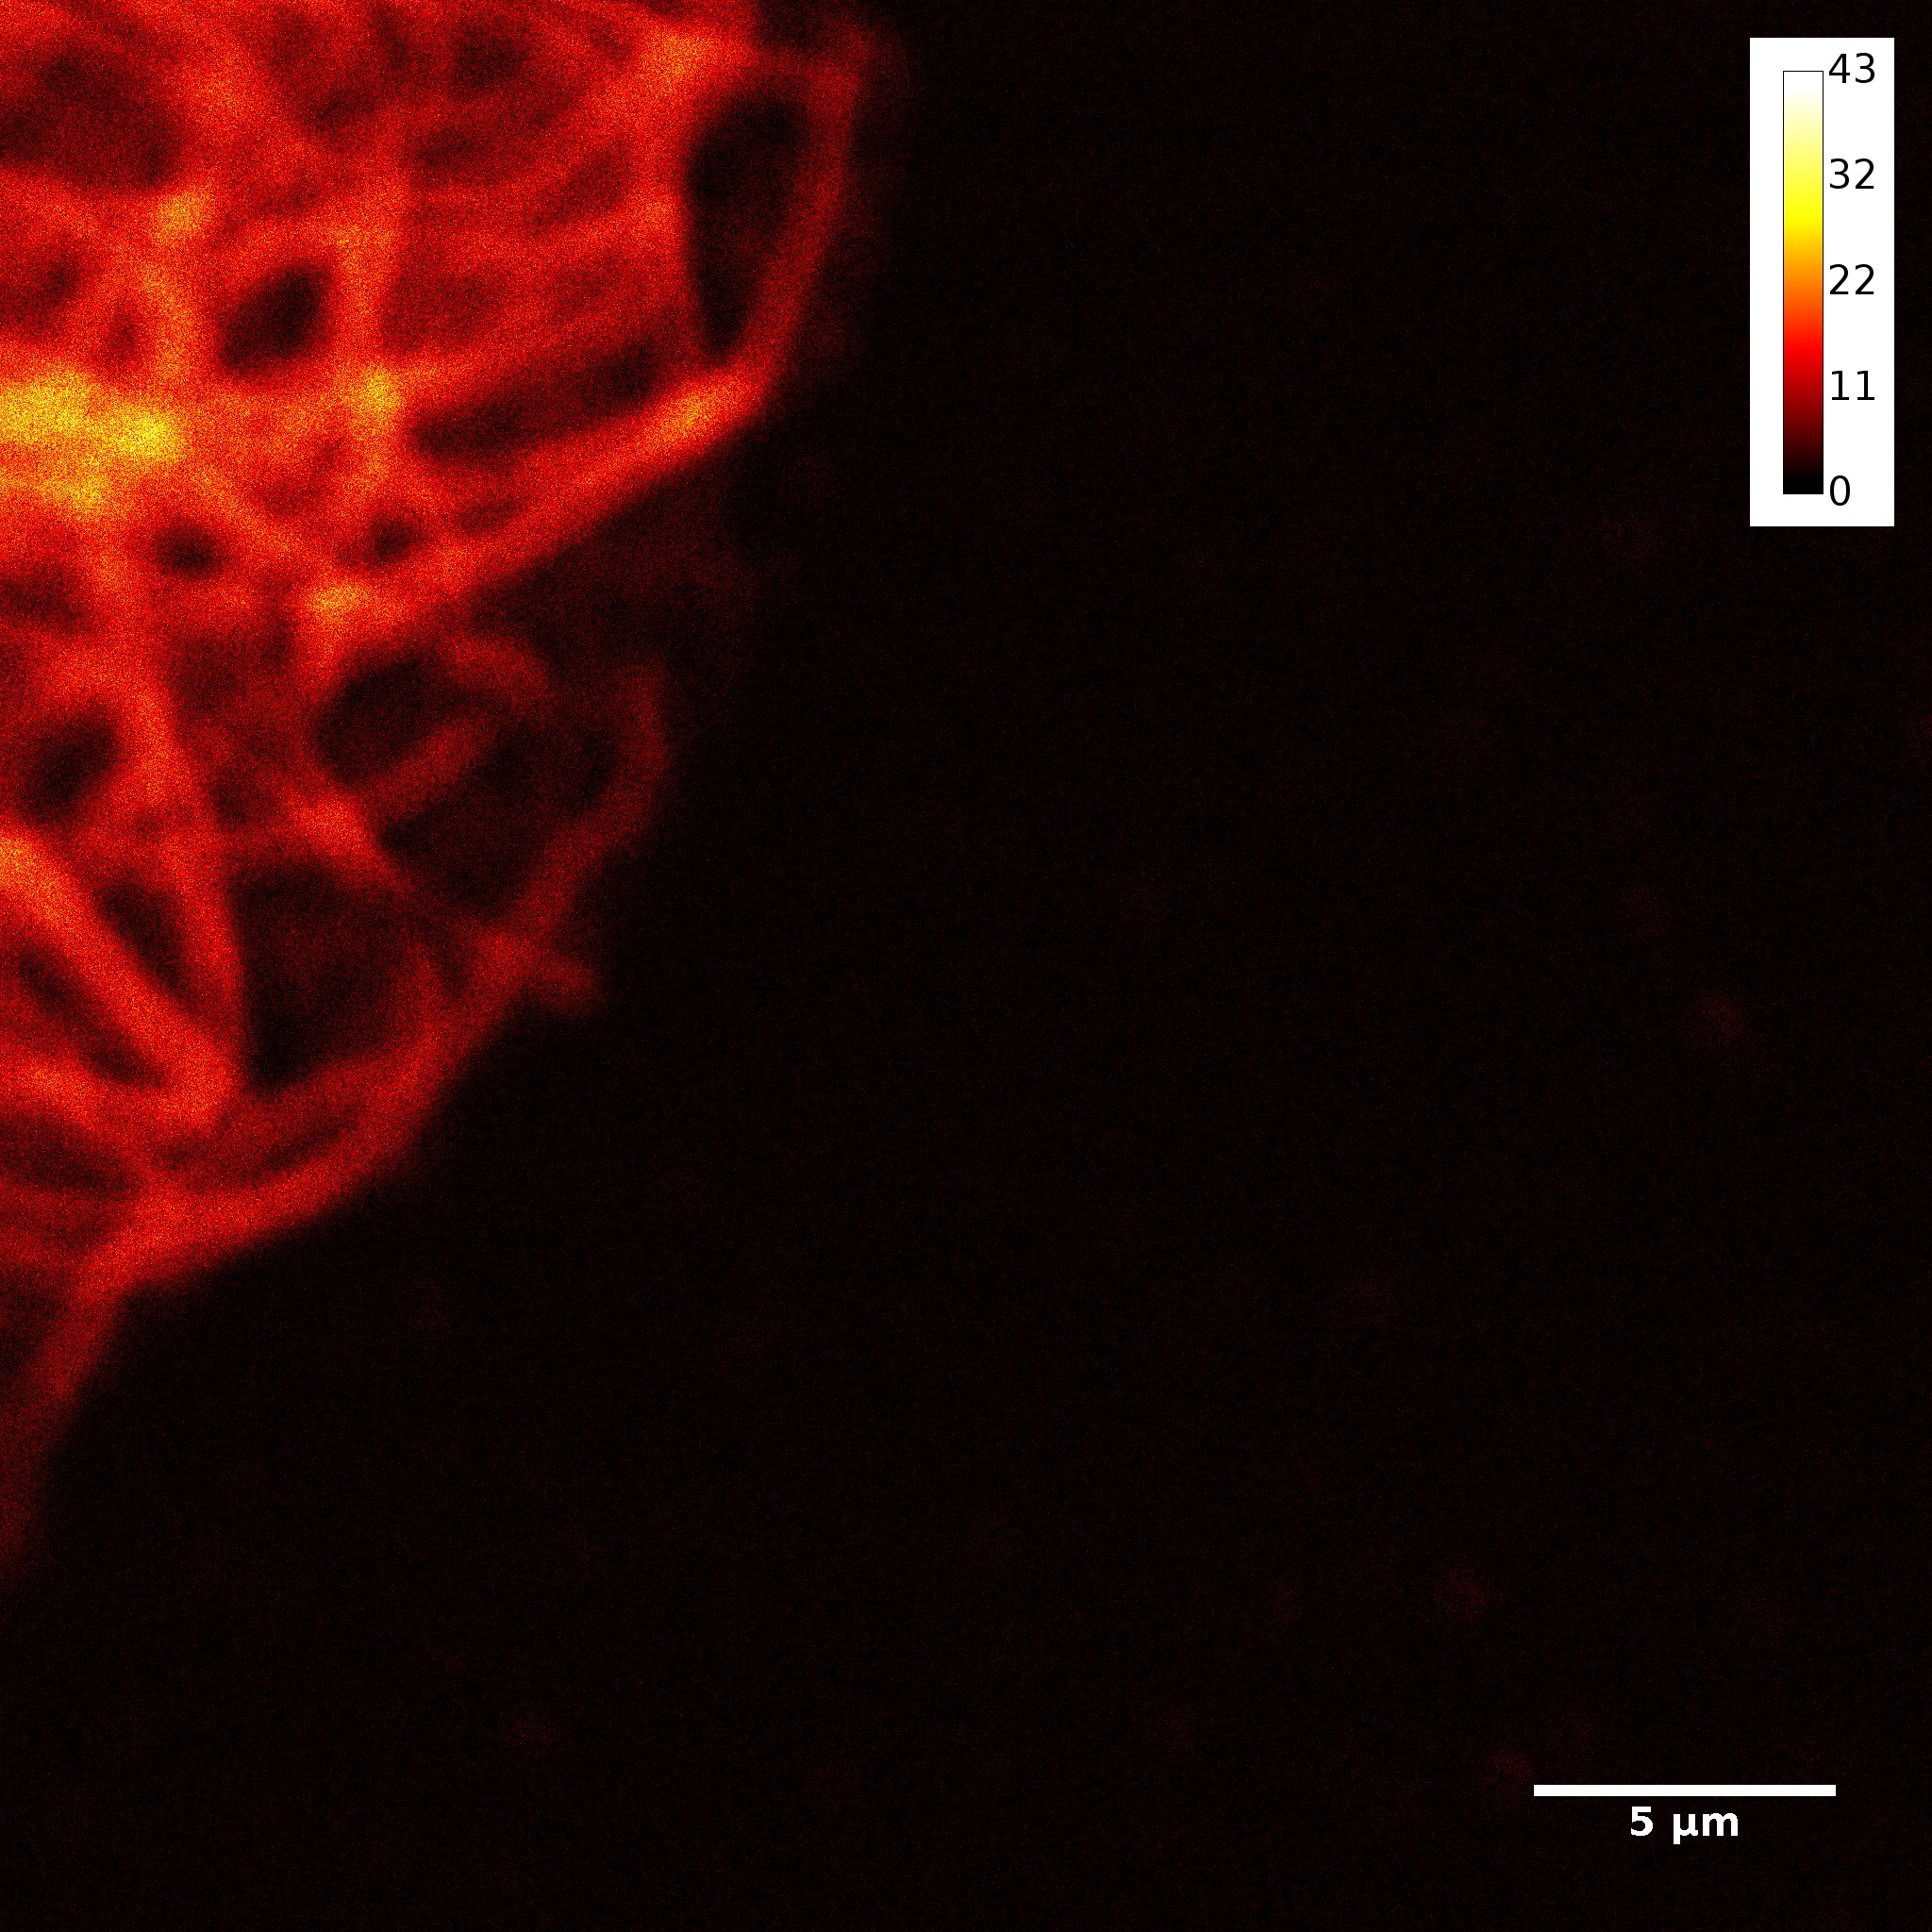
\includegraphics[width=\textwidth]{plots/normal_onlySTED_measurement_with_bar.jpg}
	\caption{STED-Laser allein.}\label{fig:onlysted}
\end{subfigure}
~
\begin{subfigure}{0.3\textwidth}
	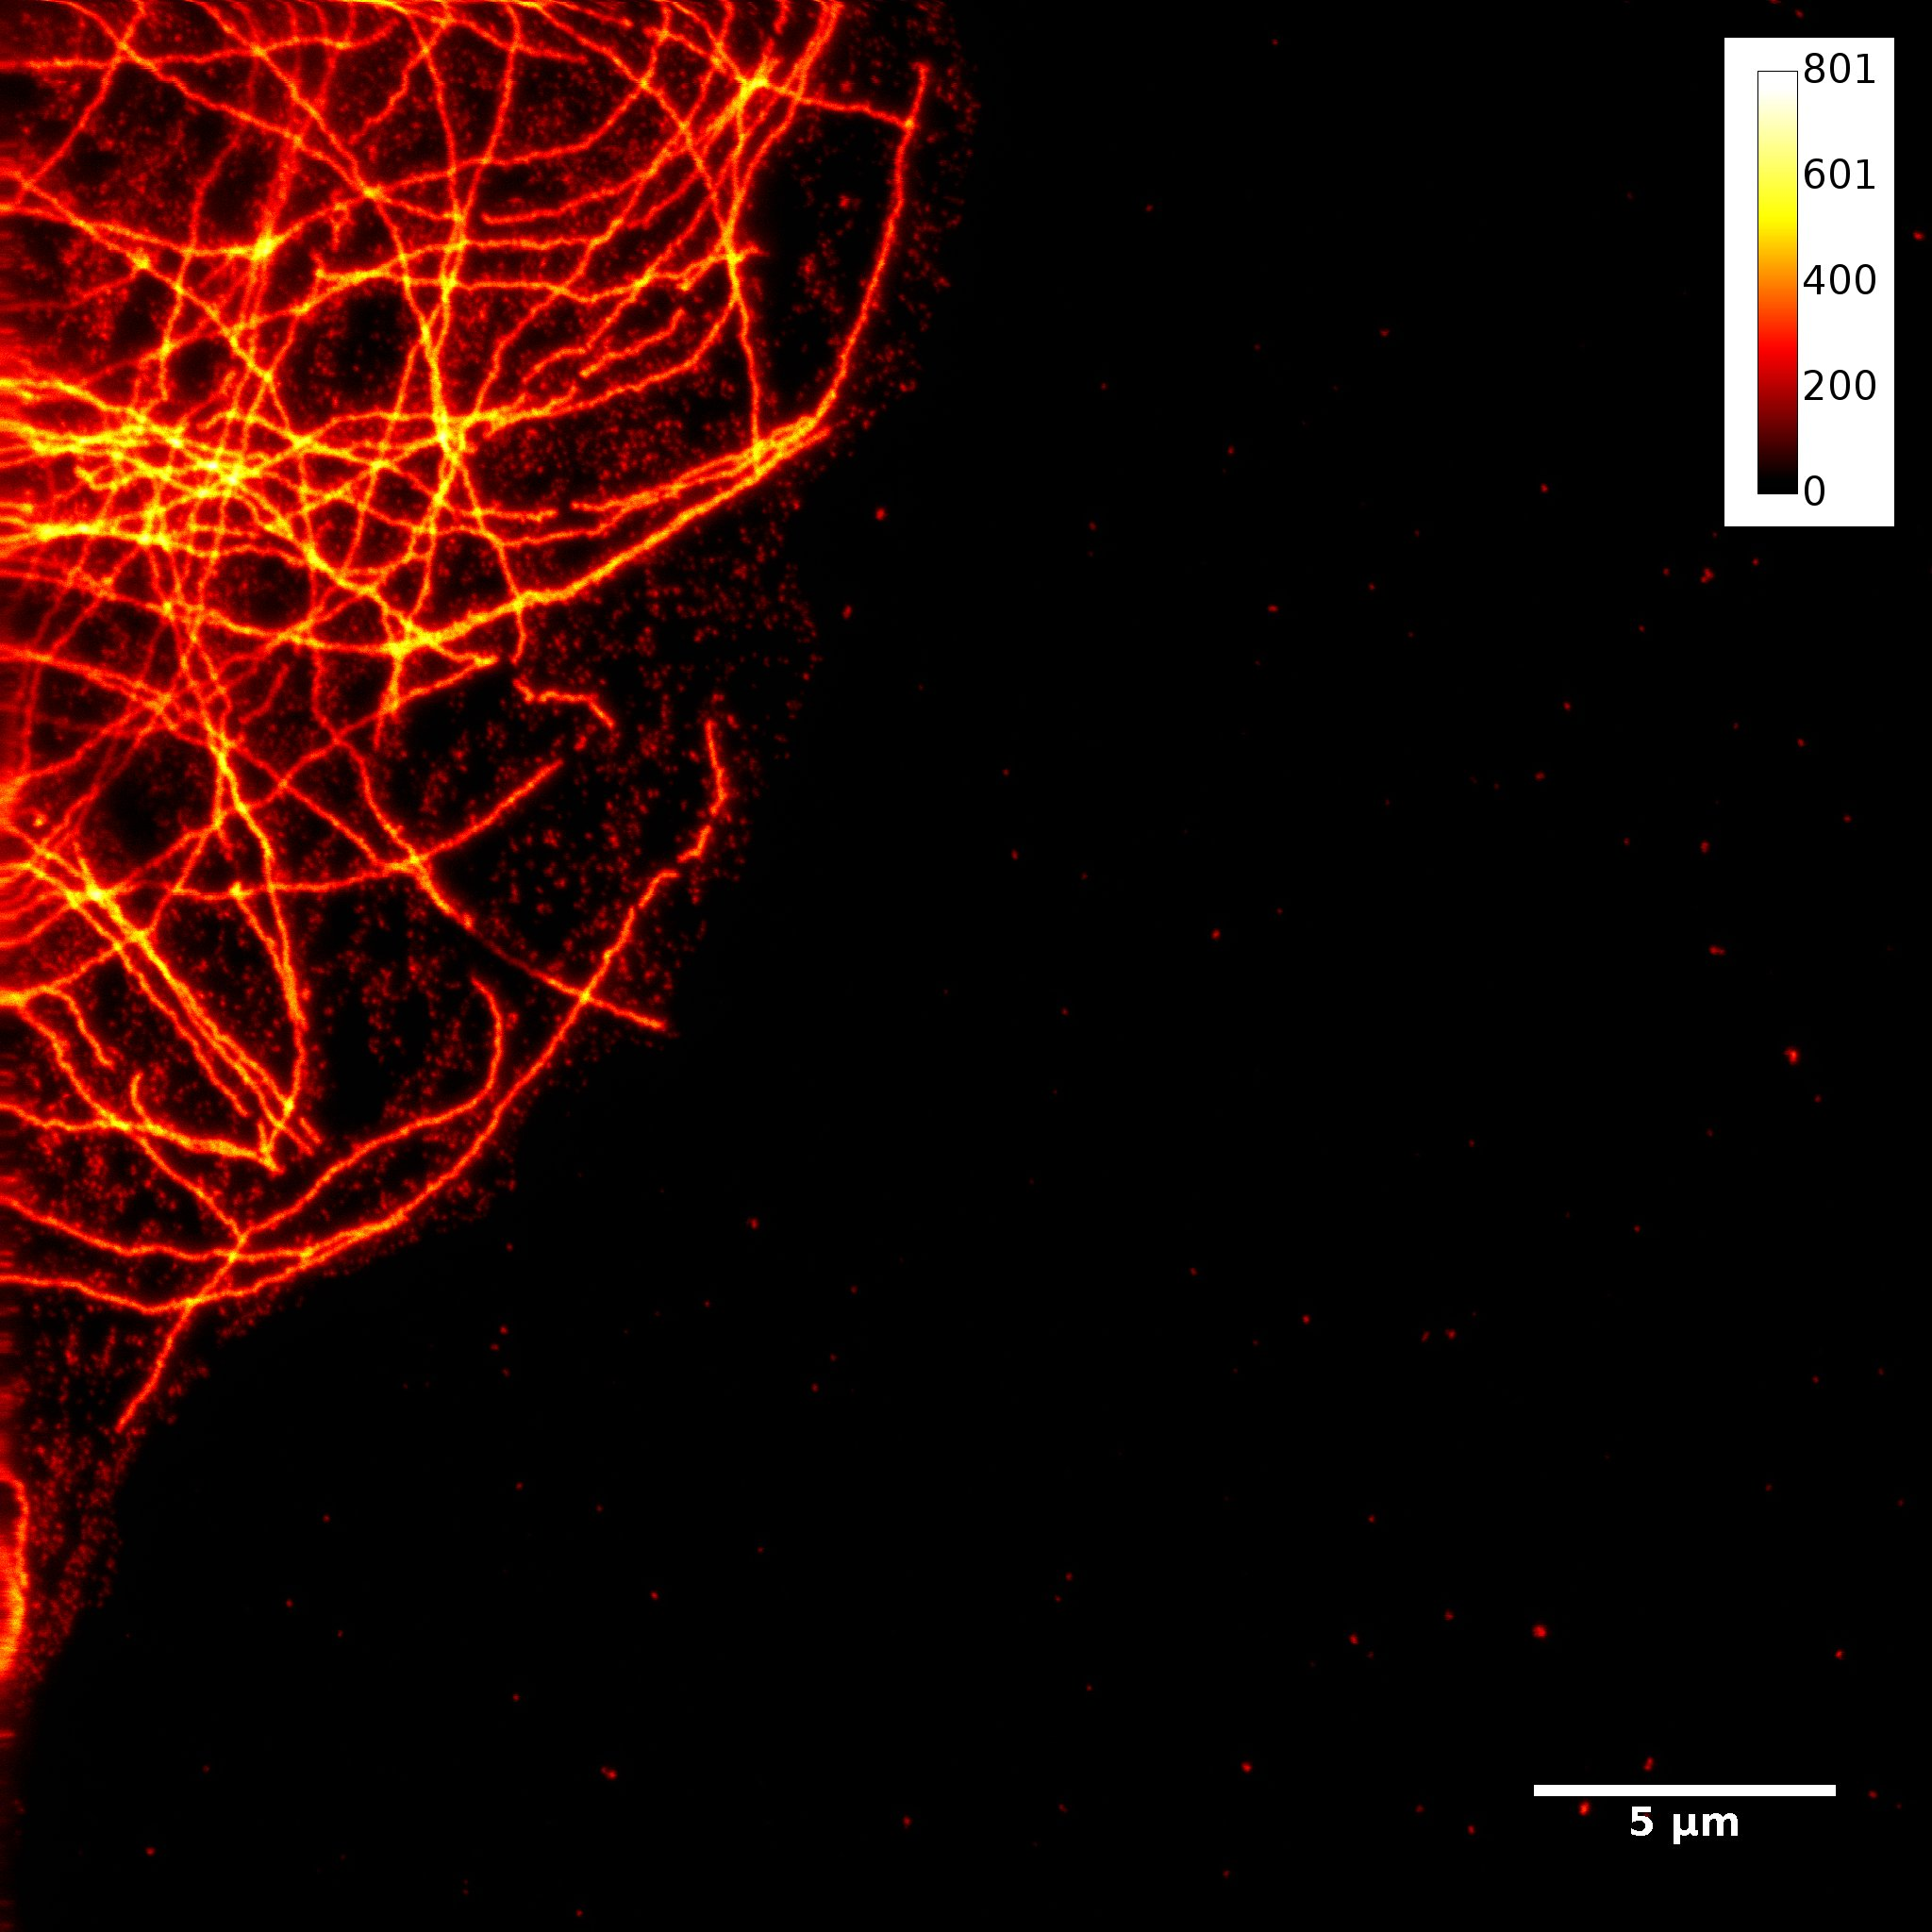
\includegraphics[width=\textwidth]{plots/normal_STED_measurement_with_bar.jpg}
	\caption{Beide Laser.}\label{fig:tubuli_sted}
\end{subfigure}
\caption{Aufnahmen von Mikrotubuli für unterschiedliche Beleuchtungen.}
\end{figure}
